% ============================================================
%  hw4_sol_numerical.tex  --  MATH 6660, Homework 4,
%  Problems 1, 2, 3 (PyDistMesh + cG(1) on the star) and 4(d) (bilinear
%  squares on [-1,1]^2).
%
%  RULE: nothing here goes beyond the class lectures.  Anything that
%  would is wrapped in \outside{}{} and prints as a red labelled box.
%
%  Every table and figure is written by a script in this folder:
%     hw4_p1_pydistmesh.py   -> hw4_p1_examples.pdf, hw4_p1_table.tex
%     hw4_p23_star.py        -> hw4_p2_mesh.pdf, hw4_p2_table.tex,
%                               hw4_p3_solution.pdf, hw4_p3_table.tex,
%                               hw4_p3_disc_table.tex
%     hw4_p4d_q1.py          -> hw4_p4d_table.tex, hw4_p4d_figure.pdf
%  Equations are numbered by problem (1.1, 2.1, ..., 4d.1), so they are
%  unambiguous next to hw4_sol.pdf (Problem 4(a)-(c)).
%  Build: pdflatex hw4_sol_numerical.tex   (twice)
% ============================================================
\documentclass[11pt]{article}
\usepackage[letterpaper,margin=1in]{geometry}
\usepackage[T1]{fontenc}
\usepackage{amsmath,amssymb}
\usepackage{booktabs}
\usepackage{array}
\usepackage{graphicx}
\usepackage{caption}
\usepackage{enumitem}
\usepackage{bm}
\usepackage{xcolor}
\usepackage{xspace}
\usepackage{fancyvrb}
\usepackage[colorlinks=true,linkcolor={blue!45!black},pdfborder={0 0 0}]{hyperref}

\captionsetup{font=small,labelfont=bf,justification=justified,
              singlelinecheck=false,skip=6pt,hypcap=false}

\newcommand{\ie}{i.e.\@\xspace}
\newcommand{\dx}{\,\mathrm{d}x}
\newcommand{\dxdy}{\,\mathrm{d}x\,\mathrm{d}y}
\newcommand{\norm}[1]{\lVert #1\rVert}
\newcommand{\abs}[1]{\lvert #1\rvert}
\newcommand{\Om}{\Omega}
\newcommand{\dOm}{\partial\Omega}
\newcommand{\grad}{\nabla}
\newcommand{\lap}{\Delta}
\setlength{\parindent}{0pt}

\newcommand{\src}[1]{{\small\color{black!55}\textsf{[#1]}}}
\newcommand{\outside}[2]{%
  \par\smallskip\noindent
  \fcolorbox{red!65!black}{red!4}{%
    \parbox{0.955\linewidth}{\small
      \textbf{\color{red!65!black}NOT FROM LECTURE --- #1}\par\smallskip #2}}%
  \par\smallskip}

\newlist{steps}{itemize}{1}
\setlist[steps]{label=\textbullet, leftmargin=1.25em, topsep=3pt,
                itemsep=4pt, parsep=0pt}

% one section per problem; equations numbered <problem>.<n>
\newcommand{\problem}[2]{%
  \section*{Problem #1}%
  \renewcommand{\theequation}{#2.\arabic{equation}}%
  \setcounter{equation}{0}}

\begin{document}

% ==================================================================
\problem{1}{1}

\textbf{Problem.} Download the PyDistMesh mesh generator.  You can find all the
necessary links from the Math 6660 Canvas page.

\begin{steps}
\item Downloaded from Canvas.  PyDistMesh is B.~Froehle's Python port (2012)
      of P.-O.~Persson's \textsc{DistMesh} (2004).  Nothing in it was edited.
\end{steps}

\begin{center}
\begin{minipage}{\linewidth}
\centering\footnotesize
\begin{tabular}{@{}>{\raggedright\arraybackslash}p{0.27\linewidth}>{\raggedright\arraybackslash}p{0.69\linewidth}@{}}
\toprule
file & role\\
\midrule
\texttt{distmesh2d.py} & \texttt{p,t = distmesh2d(fd,fh,h0,bbox,pfix)}: level set
  \texttt{fd}, relative size \texttt{fh}, edge length \texttt{h0}; returns
  nodes \texttt{p} ($N\times2$) and triangles \texttt{t} ($M\times3$)\\
\texttt{distance\_functions.py} & level sets (\texttt{dcircle},
  \texttt{drectangle}, \dots) and Booleans: \texttt{dunion} $=\min$,
  \texttt{dintersect} $=\max$, \texttt{ddiff}$(d_1,d_2)=\max(d_1,-d_2)$\\
\texttt{boundary.py} & \texttt{bnd2d}: re-triangulates, marks nodes with
  $\abs{\phi}\le10^{-8}$ as boundary and puts them last, returns the areas\\
\texttt{assemble.py} & the cG(1) code used in Problem 3\\
\texttt{example1.py}, \texttt{example2.py}, \texttt{poisson\_example.py} &
  unit disc; square with a hole, graded; $-\lap u=1$ on the latter\\
\bottomrule
\end{tabular}
\captionof{table}{The PyDistMesh bundle as downloaded (plus two helper files,
\texttt{utils.py} and \texttt{mlcompat.py}).}
\label{tab:p1files}
\end{minipage}
\end{center}

\subsection*{Step 1 --- what in the code is the lecture
  \ \src{Lecture 13, Part IV, eqs.~(1.278)--(1.282)}}

\begin{steps}
\item \texttt{fd} is the lecture's level set $\phi$: $\dOm=\{\phi=0\}$,
      $\Om=\{\phi<0\}$.  The Booleans are the lecture's $\min$ (union) and
      $\max$ (intersection); a set difference is $\max(\phi_1,-\phi_2)$.
\item Points become triangles by the lecture's two Python lines: a
      Delaunay triangulation from \texttt{scipy.spatial}, then only the
      triangles whose centroid has $\phi<0$ are kept.
\item Areas are the lecture's $\tfrac12\abs{\underline v_1\times\underline v_2}$.
      Boundary nodes go last, so $u=0$ is imposed by assembling only the
      first \texttt{num\_int\_nodes} rows and columns.
\end{steps}

\outside{where the nodes come from}{The lecture triangulates a given point set.
\textsc{DistMesh} generates the points: a lattice of spacing $h_0$ cut to
$\phi<0$, then relaxed by treating every Delaunay edge as a compressed bar of
rest length $1.2\,\texttt{fh}$, re-triangulating as nodes move and projecting
escaped nodes back onto $\phi=0$.  Persson and Strang, \emph{SIAM Review} 46
(2004).}

\subsection*{Step 2 --- it runs}

\begin{center}
\begin{minipage}{\linewidth}
\centering
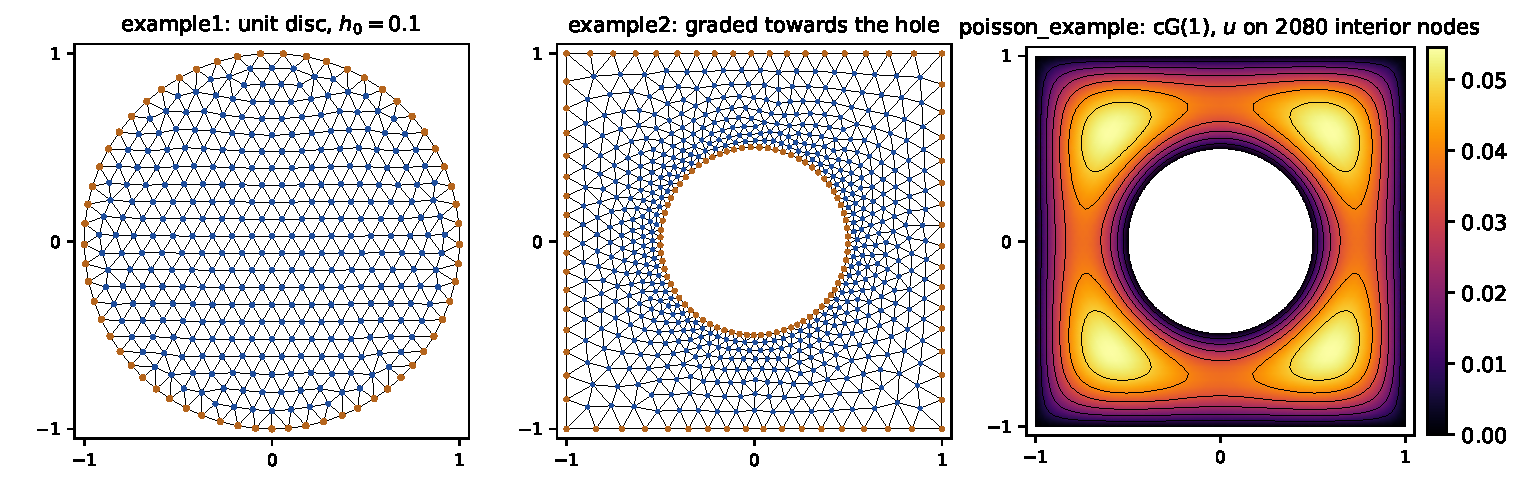
\includegraphics[width=0.86\linewidth]{hw4_p1_examples.pdf}
\captionof{figure}{The three bundled examples, run unchanged.  Interior nodes
blue, boundary nodes brown.  Right: the cG(1) solution of $-\lap u=1$, $u=0$
on $\dOm$.}
\label{fig:p1}
\end{minipage}
\end{center}

\begin{center}
\begin{minipage}{\linewidth}
\centering\footnotesize\setlength{\tabcolsep}{4pt}
\begin{tabular}{@{}lrrrrrrr@{}}
\toprule
example & $h_0$ & interior & boundary & elements & mesh area & exact & $\max_j h_j/\rho_j$\\
\midrule
unit disc, uniform & 0.10 & 301 & 61 & 661 & 3.1359 & 3.1416 & 2.52\\
square with hole, graded & 0.04 & 532 & 142 & 1206 & 3.2156 & 3.2146 & 2.83\\
square with hole, uniform, Poisson & 0.04 & 2080 & 291 & 4451 & 3.2155 & 3.2146 & 2.64\\
\bottomrule
\end{tabular}

\captionof{table}{The three runs.  Exact area: $\pi$ for the disc,
$4-\pi/4$ for the square with a hole of radius $1/2$.  Last column: the
lecture's regularity ratio (1.260), longest edge over inscribed diameter; an
equilateral triangle gives $\sqrt3=1.73$.}
\label{tab:p1runs}
\end{minipage}
\end{center}

\begin{steps}
\item Areas agree to $0.2\%$; the disc comes out smaller and the holed
      square larger, since chords cut a sliver off a convex boundary and add
      one at a concave one.  $\max_j h_j/\rho_j\le2.83$: no slivers.
\end{steps}

% ==================================================================
\problem{2}{2}

\textbf{Problem.} Use this code to generate a mesh for a star-shaped region
whose boundary is the zero contour of $\phi(r,\theta)=r-0.75-0.25\sin(5\theta)$.

\subsection*{Step 1 --- the level set in $x,y$
  \ \src{Lecture 13, eqs.~(1.279)--(1.280)}}

\begin{steps}
\item \texttt{fd} receives Cartesian points, so with $r=\sqrt{x^{2}+y^{2}}$,
      $\theta=\operatorname{atan2}(y,x)$:
\begin{equation}\label{eq:phi}
  \begin{gathered}
  \phi(x,y)=\sqrt{x^{2}+y^{2}}-0.75-0.25\sin\bigl(5\operatorname{atan2}(y,x)\bigr),\\
  \phi<0\iff r<R(\theta):=0.75+0.25\sin5\theta .
  \end{gathered}
\end{equation}
      $0.5\le R\le1$: five tips at $r=1$, five valleys at $r=0.5$; the box
      $(-1,1)^{2}$ contains $\Om$.
\begin{Verbatim}[fontsize=\small,xleftmargin=1em]
fd = lambda p: np.sqrt(p[:,0]**2 + p[:,1]**2) - 0.75 \
               - 0.25*np.sin(5*np.arctan2(p[:,1], p[:,0]))
p, t = dm.distmesh2d(fd, distfunc.huniform, h0, (-1,-1,1,1))
p, t, nin, nbd, area = bnd.bnd2d(fd, p, t, -1.0, -1.0, 1.0, 1.0)
\end{Verbatim}
\item Exact area, to check the mesh against:
\begin{equation}\label{eq:area}
  \abs{\Om}=\int_{0}^{2\pi}\!\!\int_{0}^{R(\theta)}r\,\mathrm{d}r\,\mathrm{d}\theta
  =\frac12\int_{0}^{2\pi}\Bigl[0.75^{2}+1.5\cdot0.25\underbrace{\sin5\theta}_{\int=\,0}
   +0.25^{2}\underbrace{\sin^{2}5\theta}_{\int=\,\pi}\Bigr]\mathrm{d}\theta
  =\frac{19\pi}{32}=1.86532 .
\end{equation}
\end{steps}

\subsection*{Step 2 --- the boundary nodes, and a fix}

\begin{steps}
\item \texttt{bnd2d} calls a node \emph{boundary} only if
      $\abs{\phi}\le10^{-8}$, and Problem 3's solver sets $u=0$ only there.
      So every node on a boundary edge (an edge of one triangle only) must
      pass that test.
\item \textbf{It does not.}  At $h_0=0.05$ only $72$ of the $138$ nodes on
      boundary edges pass (Table~\ref{tab:p2}, last column).  The $66$ others
      sit just inside, $-1.0\times10^{-4}\le\phi<-10^{-8}$, all on the inner
      part of the boundary, $r\le0.78$, around the five valleys
      (Figure~\ref{fig:p2}, red).
\item \textbf{Why.}  \texttt{distmesh2d} moves a node that left $\Om$ back by
      $\bm p\leftarrow\bm p-\phi\,\grad\phi/\abs{\grad\phi}^{2}$, repeated
      \emph{while $\phi>10^{-14}$}.  One step lands exactly on $\phi=0$ only if
      $\phi$ is linear along $\grad\phi$, as for $\phi=r-1$ in the bundle's
      examples.  Here
\begin{equation}\label{eq:gradphi}
  \grad\phi=\underbrace{\bm e_{r}}_{\partial\phi/\partial r}
           \;-\;\underbrace{\frac{1.25\cos5\theta}{r}\,\bm e_{\theta}}_{\frac1r\partial\phi/\partial\theta}
\end{equation}
      is not radial, so a step can land inside, and then the loop stops with
      $\phi<0$.
\item \textbf{Fix} (the bundle is not edited).  Before \texttt{bnd2d}, move
      every node on a boundary edge radially onto the curve:
\begin{equation}\label{eq:snap}
  (x,y)\;\leftarrow\;R(\theta)\,(\cos\theta,\sin\theta),
  \qquad\text{so}\quad \phi=R(\theta)-R(\theta)=0 .
\end{equation}
      The nodes move at most $10^{-4}\ll h_{0}$.  Afterwards every boundary
      node passes (Table~\ref{tab:p2}).
\end{steps}

\subsection*{Step 3 --- the mesh
  \ \src{Lecture 13, eq.~(1.260): regular triangulation}}

\begin{center}
\begin{minipage}{\linewidth}
\centering
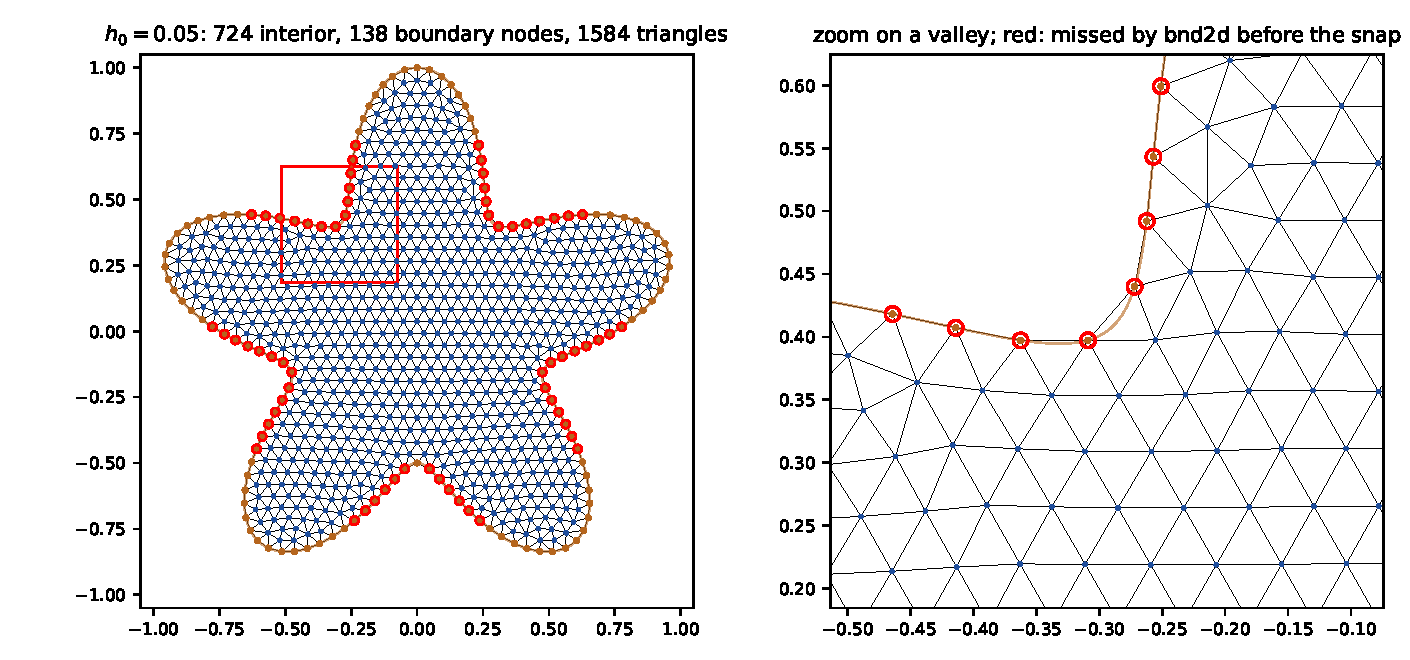
\includegraphics[width=0.97\linewidth]{hw4_p2_mesh.pdf}
\captionof{figure}{The star mesh at $h_{0}=0.05$, after the fix
\eqref{eq:snap}.  Blue: interior nodes; brown: boundary nodes; the curve is
$\phi=0$.  Red circles: the boundary nodes that \texttt{bnd2d} classed as
interior before the fix.}
\label{fig:p2}
\end{minipage}
\end{center}

\begin{center}
\begin{minipage}{\linewidth}
\centering\small\setlength{\tabcolsep}{4pt}
\begin{tabular}{@{}rrrrrrrc@{}}
\toprule
$h_0$ & interior & boundary & elements & mesh area & rel.\ error & $\max_j h_j/\rho_j$ & flagged: raw $\to$ snapped\\
\midrule
0.100 & 149 & 66 & 362 & 1.86001 & $-2.8\!\times\!10^{-3}$ & 2.57 & 32/66 $\to$ 66/66\\
0.050 & 724 & 138 & 1584 & 1.86432 & $-5.4\!\times\!10^{-4}$ & 2.46 & 72/138 $\to$ 138/138\\
0.025 & 3167 & 282 & 6614 & 1.86498 & $-1.9\!\times\!10^{-4}$ & 2.45 & 140/282 $\to$ 282/282\\
\bottomrule
\end{tabular}

\captionof{table}{Star meshes.  Exact area $19\pi/32=1.86532$
\eqref{eq:area}.  Last column: nodes \texttt{bnd2d} marks as boundary, out of
the nodes on boundary edges, before and after \eqref{eq:snap}.}
\label{tab:p2}
\end{minipage}
\end{center}

\begin{steps}
\item The area error falls from $0.3\%$ to $0.02\%$ as $h_{0}$ goes from
      $0.1$ to $0.025$.
\item $\max_{j}h_{j}/\rho_{j}\le2.57$ on every mesh (equilateral: $1.73$):
      regular in the sense of (1.260), no slivers in the valleys.
\end{steps}

% ==================================================================
\problem{3}{3}

\textbf{Problem.} Use the CG(1) method developed in class and provided on the
Math 6660 Canvas page to solve $-u_{,xx}-u_{,yy}=1$ in $\Om$, $u=0$ on $\dOm$,
on the star of Problem 2.

\subsection*{Step 1 --- the method
  \ \src{Lecture 13, eqs.~(1.236) and (1.253)--(1.255)}}

\begin{steps}
\item Weak form: find $u\in H^{1}_{0}(\Om)$ with
      $\iint_{\Om}\grad u\cdot\grad v\dxdy=\iint_{\Om}f v\dxdy$ for all $v$,
      $f=1$.
\item $V_{h}$: continuous, linear on each triangle of Problem 2, zero at the
      boundary nodes.  Basis: the hat $\varphi_{i}$ of each interior node.
      $U=\sum_{i}\xi_{i}\varphi_{i}$ and
      $\bm A\bm\xi=\bm b$ with $A_{ij}=\iint\grad\varphi_{i}\cdot\grad\varphi_{j}$,
      $b_{j}=\iint f\varphi_{j}$.
\end{steps}

\subsection*{Step 2 --- what \texttt{assemble.py} computes, triangle by triangle}

\begin{steps}
\item On a triangle $K$ with vertices $(x_{l},y_{l})$, $l=1,2,3$, the hat of
      vertex $k$ is $a_{k}+b_{k}x+c_{k}y$ with value $\delta_{kl}$ at vertex
      $l$:
\begin{equation}\label{eq:hatK}
  \underbrace{\begin{bmatrix}1&x_{1}&y_{1}\\1&x_{2}&y_{2}\\1&x_{3}&y_{3}\end{bmatrix}}_{\bm M}
  \begin{bmatrix}a_{k}\\b_{k}\\c_{k}\end{bmatrix}=\bm e_{k}
  \quad\Longrightarrow\quad
  (a_{k},b_{k},c_{k})^{T}=\text{column }k\text{ of }\bm M^{-1},
\end{equation}
      and $\grad\varphi_{k}=(b_{k},c_{k})$ on $K$.
\item The gradients are constant on $K$, so the stiffness integral is exact:
\begin{equation}\label{eq:AK}
  \iint_{K}\grad\varphi_{j}\cdot\grad\varphi_{k}\dxdy=\abs{K}\,(b_{j}b_{k}+c_{j}c_{k}) .
\end{equation}
\item The load uses the vertex rule, Lecture 4's trapezoidal rule on a
      triangle:
\begin{equation}\label{eq:bK}
  \iint_{K}f\varphi_{k}\dxdy\approx\frac{\abs{K}}{3}\sum_{l=1}^{3}f(x_{l},y_{l})\,
  \underbrace{\varphi_{k}(x_{l},y_{l})}_{\delta_{kl}}=\frac{\abs{K}}{3}\,f(x_{k},y_{k}) .
\end{equation}
      For $f\equiv1$ it is exact.  $\varphi_{k}$ is linear, so its mean over
      $K$ is its value at the centroid, the average of the vertex values,
      $(1+0+0)/3$.
\item Only nodes with index below \texttt{num\_int\_nodes} get a row and a
      column: $u=0$ is built into $V_{h}$.  The assembled $\bm A$ is
      symmetric to round-off ($\max\abs{\bm A-\bm A^{T}}=0$).
\end{steps}

\subsection*{Step 3 --- check on a domain with a known answer}

\begin{steps}
\item Unit disc: $u=\tfrac14(1-x^{2}-y^{2})$ has $u_{,xx}=u_{,yy}=-\tfrac12$, so
      $-\lap u=1$, and $u=0$ at $r=1$.  Same pipeline, no fix needed: for
      $\phi=r-1$ every boundary node passes.
\end{steps}

\begin{center}
\begin{minipage}{\linewidth}
\centering\small
\begin{tabular}{@{}rrrrc@{}}
\toprule
$h_0$ & interior nodes & $\max U$ & $\max_i\abs{U_i-u(x_i,y_i)}$ & rate\\
\midrule
0.100 & 301 & 0.24983 & $4.03\!\times\!10^{-4}$ & ---\\
0.050 & 1324 & 0.24984 & $9.63\!\times\!10^{-5}$ & 2.06\\
0.025 & 5559 & 0.25000 & $2.37\!\times\!10^{-5}$ & 2.02\\
\bottomrule
\end{tabular}

\captionof{table}{The Canvas cG(1) code on the unit disc, $-\lap u=1$:
largest nodal error against $\tfrac14(1-x^{2}-y^{2})$.  It falls as
$h_{0}^{2}$.}
\label{tab:p3disc}
\end{minipage}
\end{center}

\subsection*{Step 4 --- the star}

\begin{center}
\begin{minipage}{\linewidth}
\centering
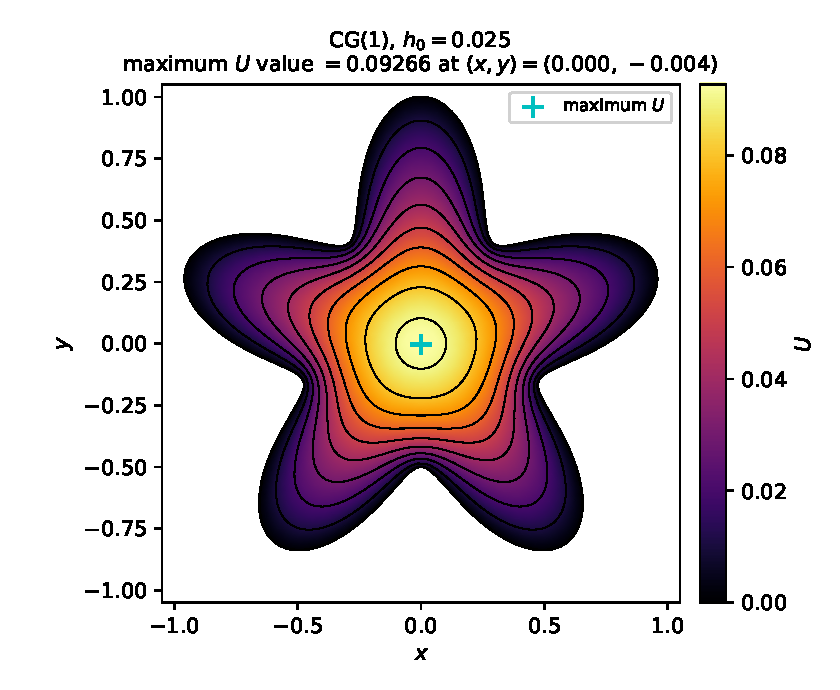
\includegraphics[width=0.5\linewidth]{hw4_p3_solution.pdf}
\captionof{figure}{cG(1) solution of $-\lap u=1$, $u=0$ on the star,
$h_{0}=0.025$ ($3167$ unknowns), with ten contours.  Cross: the largest nodal
value.}
\label{fig:p3}
\end{minipage}
\end{center}

\begin{center}
\begin{minipage}{\linewidth}
\centering\small
\begin{tabular}{@{}rrrcr@{}}
\toprule
$h_0$ & unknowns & $\max U$ & at $(x,y)$ & $\max U$, raw mesh\\
\midrule
0.100 & 149 & 0.09233 & $(0.000,\,0.032)$ & 0.23841\\
0.050 & 724 & 0.09256 & $(-0.026,\,-0.008)$ & 0.22573\\
0.025 & 3167 & 0.09266 & $(0.000,\,-0.004)$ & 0.22951\\
\bottomrule
\end{tabular}

\captionof{table}{The star under refinement.  ``Raw mesh'': the same nodes
without the fix \eqref{eq:snap} of Problem 2.}
\label{tab:p3}
\end{minipage}
\end{center}

\begin{steps}
\item $\max U=0.0927$, at the node nearest the centre --- where the five-fold
      symmetry puts it --- and stable to three digits from $h_{0}=0.05$.
\item Without the fix, $\max U\approx0.23$: the nodes missed in Problem 2 are
      left free, so along the valleys the code imposes no condition instead
      of $u=0$.  The solution is then wrong.
\end{steps}

\medskip
\noindent\fbox{\parbox{0.955\linewidth}{%
\textbf{Result.}  On the star, $\max u\approx0.0927$ at the centre and
$\iint_{\Om}u\dxdy\approx0.0676$ (Table~\ref{tab:p3}, Figure~\ref{fig:p3}).}}

\medskip
{\small\color{black!60}\textbf{Mechanics reading.}  A membrane of unit tension
under unit pressure, rim clamped.  The disc inscribed in the star ($r=0.5$)
deflects $1/16=0.0625$ at its centre, the circumscribed disc ($r=1$) $1/4$;
the star sits between, at $0.0927$.  The raw-mesh $0.23$ is almost the
circumscribed value: a membrane released along its valleys.}

% ==================================================================
\newpage
\problem{4(d)}{4d}

\textbf{Problem.} Use the method of 4(c) to solve $-\grad\cdot\grad u=f$ on
$\Om=[-1,1]^{2}$, $u=g$ on $\dOm$, with
\[
  f=\pi^{2}e^{\sin(\pi x)\sin(\pi y)}\bigl\{2\sin(\pi x)\sin(\pi y)
   +2\cos^{2}(\pi x)\cos^{2}(\pi y)-\cos^{2}(\pi x)-\cos^{2}(\pi y)\bigr\},
  \qquad g=1 .
\]
Create a convergence table showing both $\norm{\cdot}_{V}$ and
$\norm{\cdot}_{L^{2}(\Om)}$ errors.  What order of convergence do you observe?
The exact solution is $u=e^{\sin(\pi x)\sin(\pi y)}$.

\subsection*{Step 1 --- the data are consistent}

\begin{steps}
\item With $s=\sin\pi x\sin\pi y$ and $u=e^{s}$,
      $u_{,x}=\pi\cos\pi x\sin\pi y\,e^{s}$ and
\begin{align}
  -u_{,xx}-u_{,yy}
  &=\pi^{2}e^{s}\bigl[2\sin\pi x\sin\pi y
     -\cos^{2}\!\pi x\,\underbrace{\sin^{2}\!\pi y}_{1-\cos^{2}\pi y}
     -\underbrace{\sin^{2}\!\pi x}_{1-\cos^{2}\pi x}\cos^{2}\!\pi y\bigr]\notag\\
  &=\pi^{2}e^{s}\bigl[2\sin\pi x\sin\pi y+2\cos^{2}\!\pi x\cos^{2}\!\pi y
     -\cos^{2}\!\pi x-\cos^{2}\!\pi y\bigr]=f .\label{eq:lap}
\end{align}
      Also checked symbolically ($-\lap u-f\equiv0$).
\item On every side $\sin(\pm\pi)=0$, so $s=0$ and $u=e^{0}=1=g$.
\end{steps}

\subsection*{Step 2 --- the implementation \ \src{4(c); Lecture 5, eq.~(1.66)}}

\begin{steps}
\item \textbf{Grid.}  $N\times N$ squares, $N=4,\dots,256$, $h=2/N$,
      $(N-1)^{2}$ unknowns.
\item \textbf{Stiffness.}  The element matrix $\bm k^{e}$ of 4(c), the same on
      every square, assembled.  Checked in the code: every interior row is
      the stencil $\tfrac13[8;\,-1\times8]$ of 4(c), the interior matrix is
      symmetric positive definite, and the boundary terms are $5/3$, $1$, $0$
      as in 4(c).
\item \textbf{Boundary.}  $U=g=1$ at boundary nodes, moved to the right-hand
      side (Lecture 5).
\item \textbf{Load.}  $b_{ij}=\iint f\varphi_{ij}$ by $3\times3$ Gauss points
      per square, not the trapezoidal $h^{2}f_{ij}$ of 4(c); Step 4 compares.
\item \textbf{Errors,} $4\times4$ Gauss points per square, with the norm of
      Lecture 13, eq.~(1.254):
\begin{equation}\label{eq:norms}
  \norm{e}_{L^{2}(\Om)}^{2}=\iint_{\Om}(u-U)^{2}\dxdy,
  \qquad
  \norm{e}_{V}^{2}=\norm{e}_{L^{2}(\Om)}^{2}+\iint_{\Om}\abs{\grad(u-U)}^{2}\dxdy .
\end{equation}
      Rate $=\log_{2}\bigl(E(h)/E(h/2)\bigr)$.
\end{steps}

\subsection*{Step 3 --- convergence table}

\begin{center}
\begin{minipage}{\linewidth}
\centering\small
\begin{tabular}{@{}rrrlclc@{}}
\toprule
$N$ & $h$ & unknowns & $\norm{e}_{V}$ & rate & $\norm{e}_{L^{2}(\Omega)}$ & rate\\
\midrule
4 & $0.50000$ & 9 & $2.1378\!\times\!10^{0}$ & --- & $2.3519\!\times\!10^{-1}$ & ---\\
8 & $0.25000$ & 49 & $1.4636\!\times\!10^{0}$ & 0.55 & $9.5737\!\times\!10^{-2}$ & 1.30\\
16 & $0.12500$ & 225 & $7.3914\!\times\!10^{-1}$ & 0.99 & $2.4256\!\times\!10^{-2}$ & 1.98\\
32 & $0.06250$ & 961 & $3.7048\!\times\!10^{-1}$ & 1.00 & $6.0808\!\times\!10^{-3}$ & 2.00\\
64 & $0.03125$ & 3969 & $1.8536\!\times\!10^{-1}$ & 1.00 & $1.5213\!\times\!10^{-3}$ & 2.00\\
128 & $0.01562$ & 16129 & $9.2693\!\times\!10^{-2}$ & 1.00 & $3.8038\!\times\!10^{-4}$ & 2.00\\
256 & $0.00781$ & 65025 & $4.6348\!\times\!10^{-2}$ & 1.00 & $9.5100\!\times\!10^{-5}$ & 2.00\\
\bottomrule
\end{tabular}

\captionof{table}{Bilinear squares on $[-1,1]^{2}$, $N\times N$ elements.}
\label{tab:p4d}
\end{minipage}
\end{center}

\begin{center}
\begin{minipage}{\linewidth}
\centering
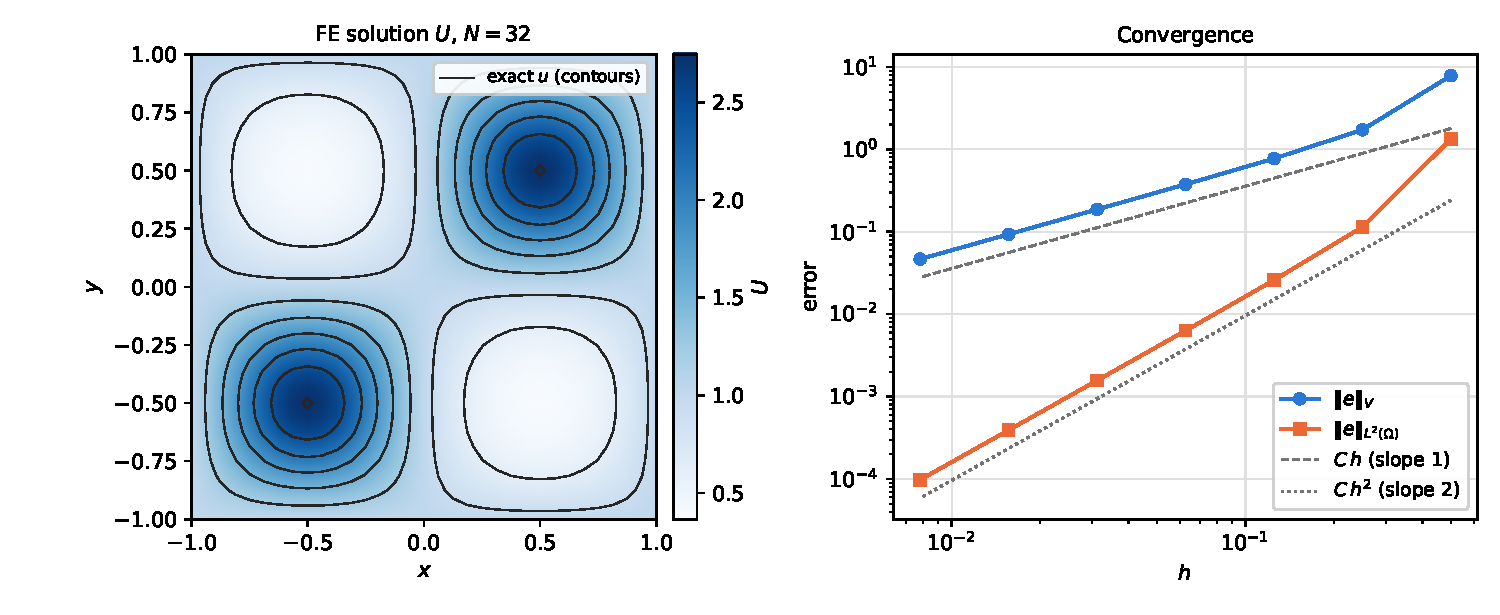
\includegraphics[width=\linewidth]{hw4_p4d_figure.pdf}
\captionof{figure}{Left: $U$ at $N=32$ with contours of the exact $u$.  Right:
the errors of Table~\ref{tab:p4d} against $h$, with slopes $1$ and $2$ for
reference.}
\label{fig:p4d}
\end{minipage}
\end{center}

\subsection*{Step 4 --- the observed orders}

\begin{steps}
\item $\norm{e}_{V}$: rate $\to1.00$, \ie $\mathcal O(h)$.
      $\norm{e}_{L^{2}(\Om)}$: rate $\to2.00$, \ie $\mathcal O(h^{2})$.  Clean
      from $N=16$; at $N=4,8$ the mesh has only two to four squares across
      each bump of $u$.
\item The trapezoidal load of 4(c) gives the same rates; at $N=256$,
      $\norm{e}_{V}=4.6355\times10^{-2}$ and
      $\norm{e}_{L^{2}}=9.7057\times10^{-5}$, against
      $4.6348\times10^{-2}$ and $9.5100\times10^{-5}$ with Gauss.
\item \textbf{Why $\mathcal O(h)$ in $\norm{\cdot}_{V}$.}  $g=1$ is reproduced
      exactly by the boundary terms of 4(c), so $U-1$ is the Galerkin
      approximation of $w=u-1\in H^{1}_{0}$, and C\'ea's lemma (Lecture 13,
      eq.~(1.242)) with the constants of 4(b) gives
\begin{equation}\label{eq:cea}
  \norm{u-U}_{V}\le\frac{\beta^{*}}{\beta_{*}}\,\norm{u-v}_{V}
  =8\,\norm{u-v}_{V}\qquad\text{for every admissible } v\in V_{h} .
\end{equation}
      With $v$ the bilinear interpolant of $u$, the right side is
      $\mathcal O(h)$.
\item \textbf{Why $\mathcal O(h^{2})$ in $L^{2}$.}  Lecture 7's duality
      argument: the interpolation estimate is used twice, once on $e$ and
      once on the dual solution, one factor of $h$ each.
\end{steps}

\outside{the interpolation estimate for squares}{Lecture 13 states
$\norm{u-u_{h}}_{H^{1}}\le c\,\norm{h\,u}_{H^{2}}$, eq.~(1.262), for linear
triangles.  The same $\mathcal O(h)$ bound for the bilinear interpolant on
squares, and the 2D duality argument behind $\mathcal O(h^{2})$ in $L^{2}$, are
standard but were not shown in class.  Table~\ref{tab:p4d} confirms both
rates.}

\medskip
\noindent\fbox{\parbox{0.955\linewidth}{%
\textbf{Conclusion.}  Bilinear squares converge at $\mathcal O(h)$ in
$\norm{\cdot}_{V}$ and $\mathcal O(h^{2})$ in $\norm{\cdot}_{L^{2}(\Om)}$ ---
the same orders as CG(1) --- with $\norm{e}_{V}=4.63\times10^{-2}$ and
$\norm{e}_{L^{2}}=9.51\times10^{-5}$ at $N=256$.}}

\end{document}
